\section{Toolflow} \label{sec5}
\noindent
We have built an end-to-end tool in Python for code replacement attack detection.
The tool takes in a set of control loop descriptions, computes their intersection and 
implements the cycle detection step. The tool has been applied to a number of small 
examples of synthetic control applications and their variants. The time taken for
the tool to run on a QuadCore Intel machine is in the order of milliseconds, and the
peak memory consumption is of the order of Kilobytes. Due to the lack of standard open
source benchmarks in this domain, we have not been yet able to check the performance of
our tool on more non-trivial benchmarks. 
% % % An overview of our tool is depicted in Fig \ref{tool_algorithm}.
% % % 
% % % \begin{figure}
% % % \begin{center}
% % % 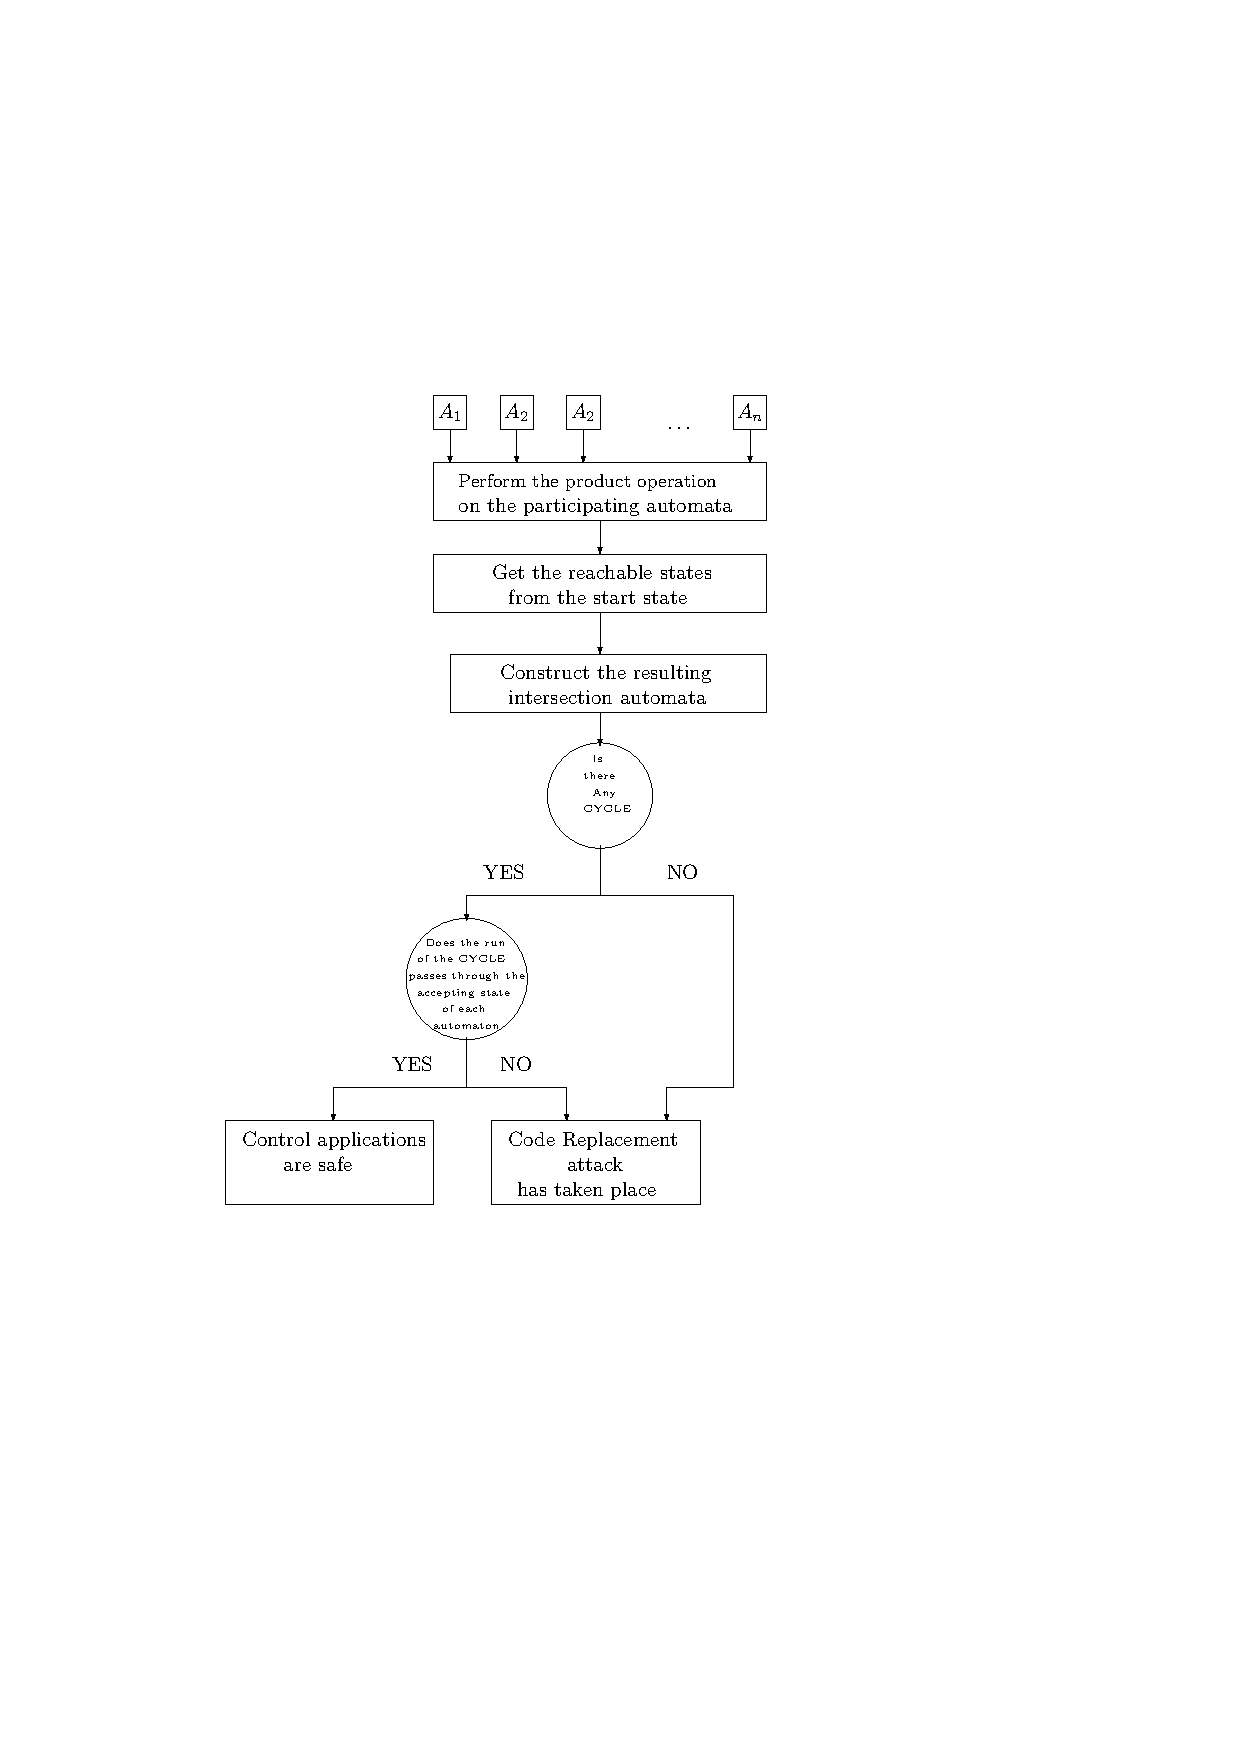
\includegraphics[width=50mm]{algorithm.pdf}
% % % \end{center}
% % % %\vspace{-0.1in}
% % % \caption{{\em The Tool flow}}
% % % \label{tool_algorithm}
% % % \end{figure}
